\documentclass{article}
\usepackage{booktabs}
\usepackage{graphicx}

\title{Regional Income Shocks: An Rcpp Simulation Toy Example}
\author{A. Author}

\begin{document}
\maketitle

\section{Introduction}

This short paper simulates region-level income shocks around a
per-region anchor income. The anchor incomes are picked from a small
household survey (\texttt{code/stata/prep\_survey.do}, one respondent
per region) and perturbed by simulated draws computed in a compiled
Rcpp routine (\texttt{src/shocks.cpp}, called from
\texttt{code/simulate.R}), producing Table~\ref{tab:main} and
Figure~\ref{fig:shocks}.

\section{Results}

\begin{table}[h]
\centering
\begin{tabular}{lc}
\toprule
Simulated mean income shock & 0.4799 \\
Simulated SD income shock & 1.0296 \\
\bottomrule
\end{tabular}


\caption{Simulated income shocks, summary statistics}
\label{tab:main}
\end{table}

\begin{figure}[h]
\centering
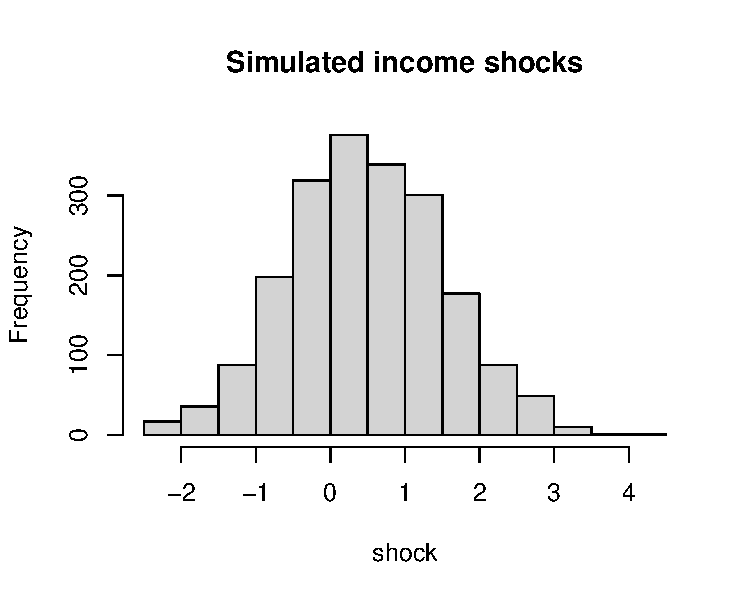
\includegraphics[width=0.6\textwidth]{output/fig1.pdf}
\caption{Distribution of simulated income shocks}
\label{fig:shocks}
\end{figure}

\end{document}
